%----------------------------------------------------------------------------------------
%    PACKAGES AND THEMES
%----------------------------------------------------------------------------------------

\documentclass[aspectratio=169,xcolor=dvipsnames]{beamer}
\usetheme{SimplePlus}

\usepackage{hyperref}
\usepackage{graphicx} % Allows including images
\usepackage{booktabs} % Allows the use of \toprule, \midrule and \bottomrule in tables
\usepackage{subcaption}

%----------------------------------------------------------------------------------------
%    TITLE PAGE
%----------------------------------------------------------------------------------------

\title{Related Rates}

\author{Colby Cox}

\institute
{
    University of Central Arkansas % Your institution for the title page
}
\date{April 18, 2025} % Date, can be changed to a custom date

%----------------------------------------------------------------------------------------
%    PRESENTATION SLIDES
%----------------------------------------------------------------------------------------

\begin{document}

\begin{frame}
  \titlepage
\end{frame}

\begin{frame}{Another Example}
  \begin{center}
    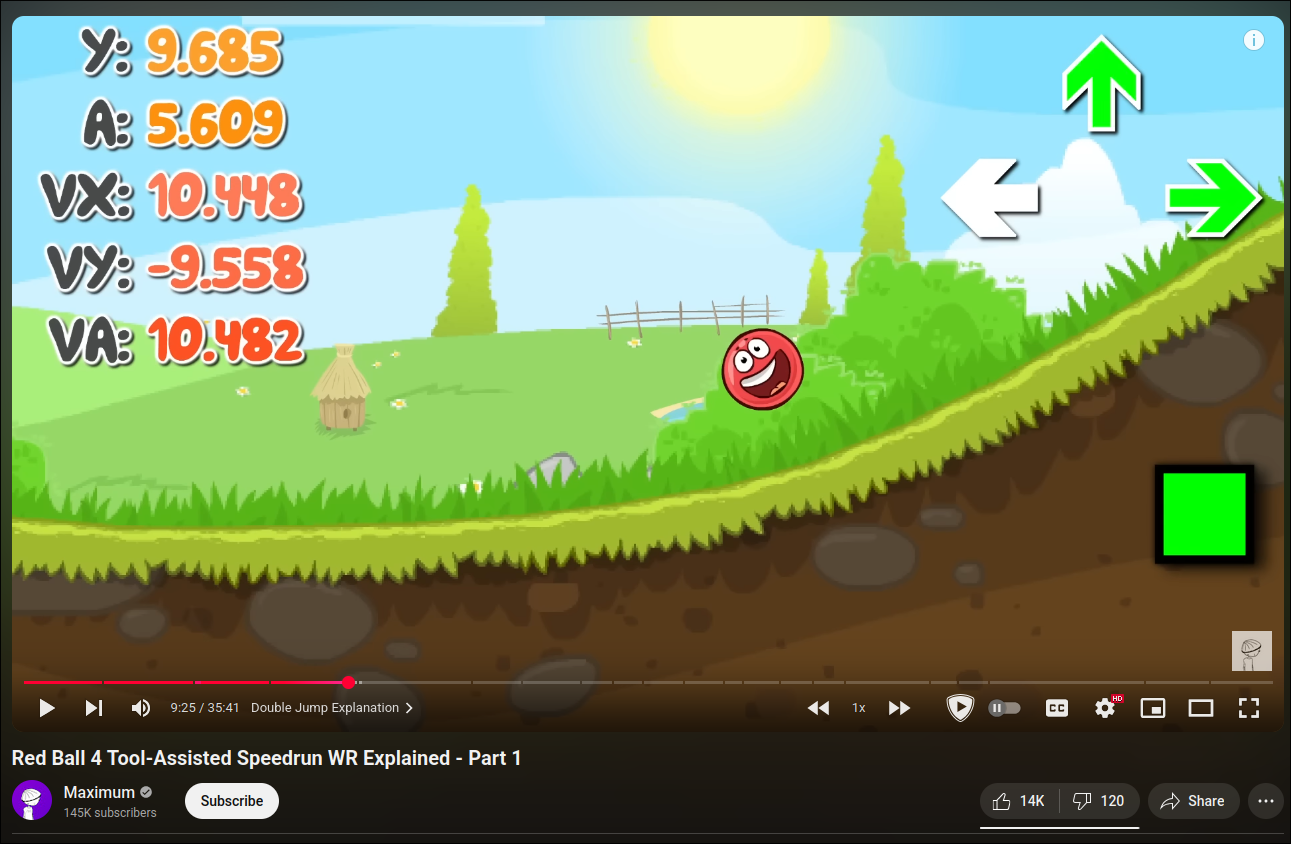
\includegraphics[scale=0.2]{redBall.png}
  \end{center}
\end{frame}

\begin{frame}{Website Renaissance}
  \begin{center}
    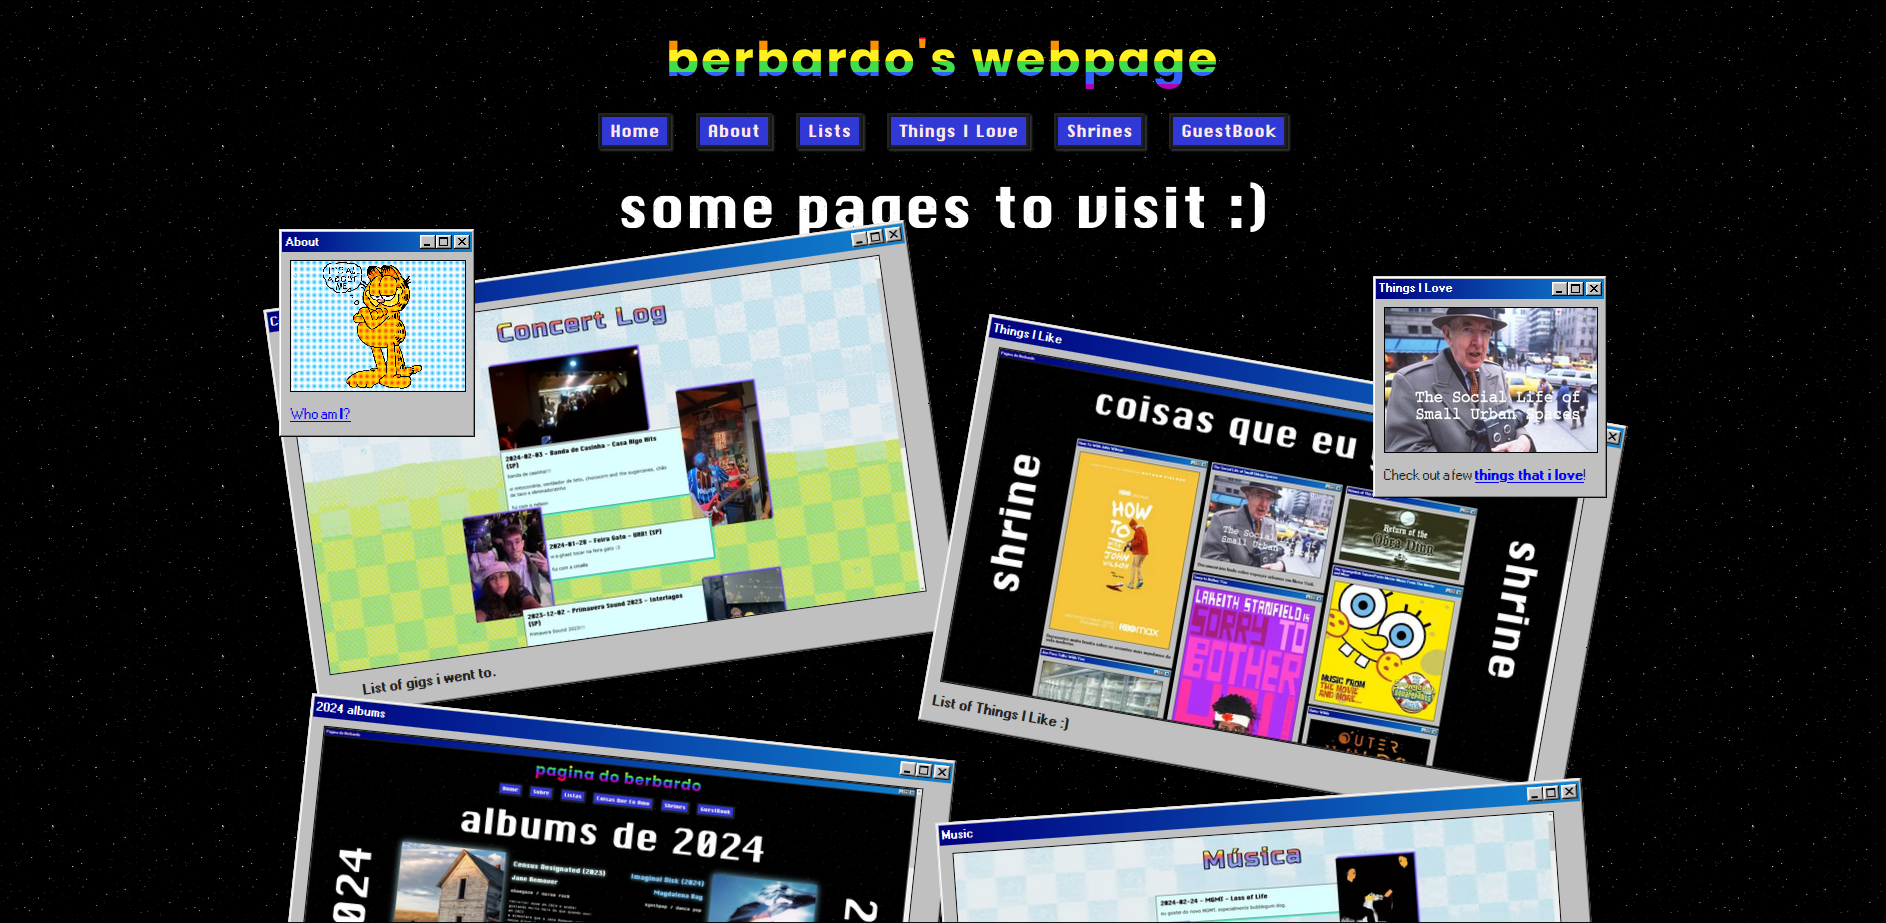
\includegraphics[scale=0.1]{website1.png}
    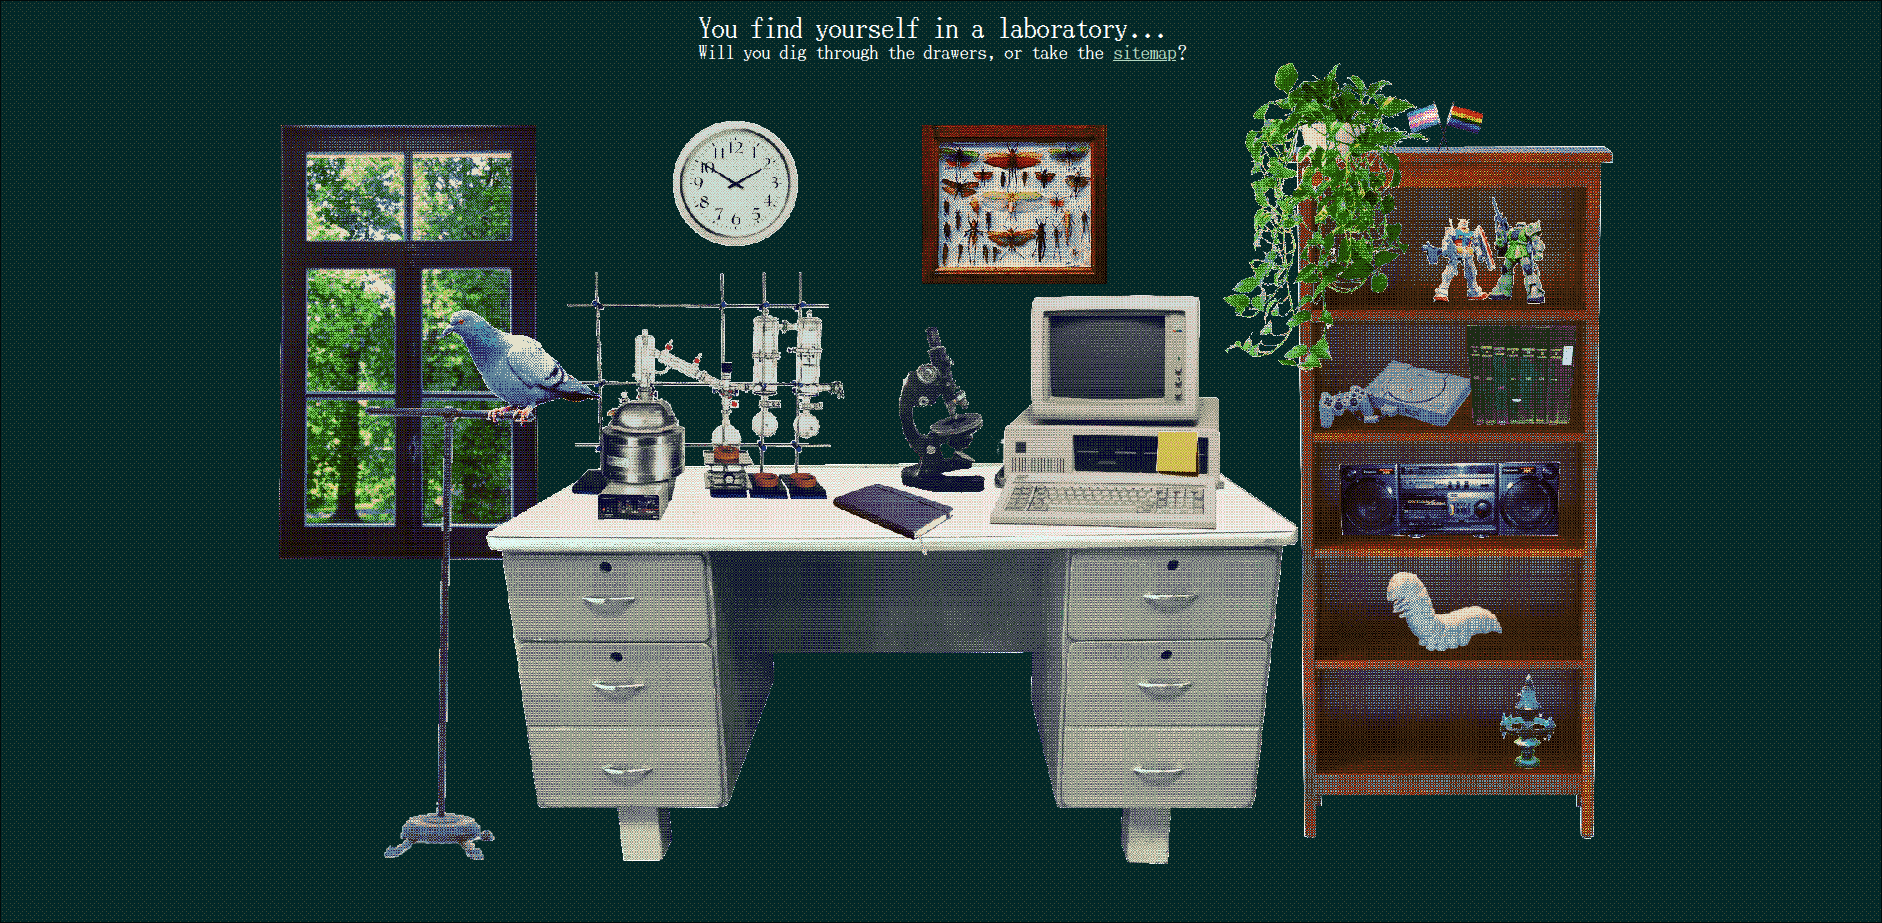
\includegraphics[scale=0.1]{website2.png}\\
    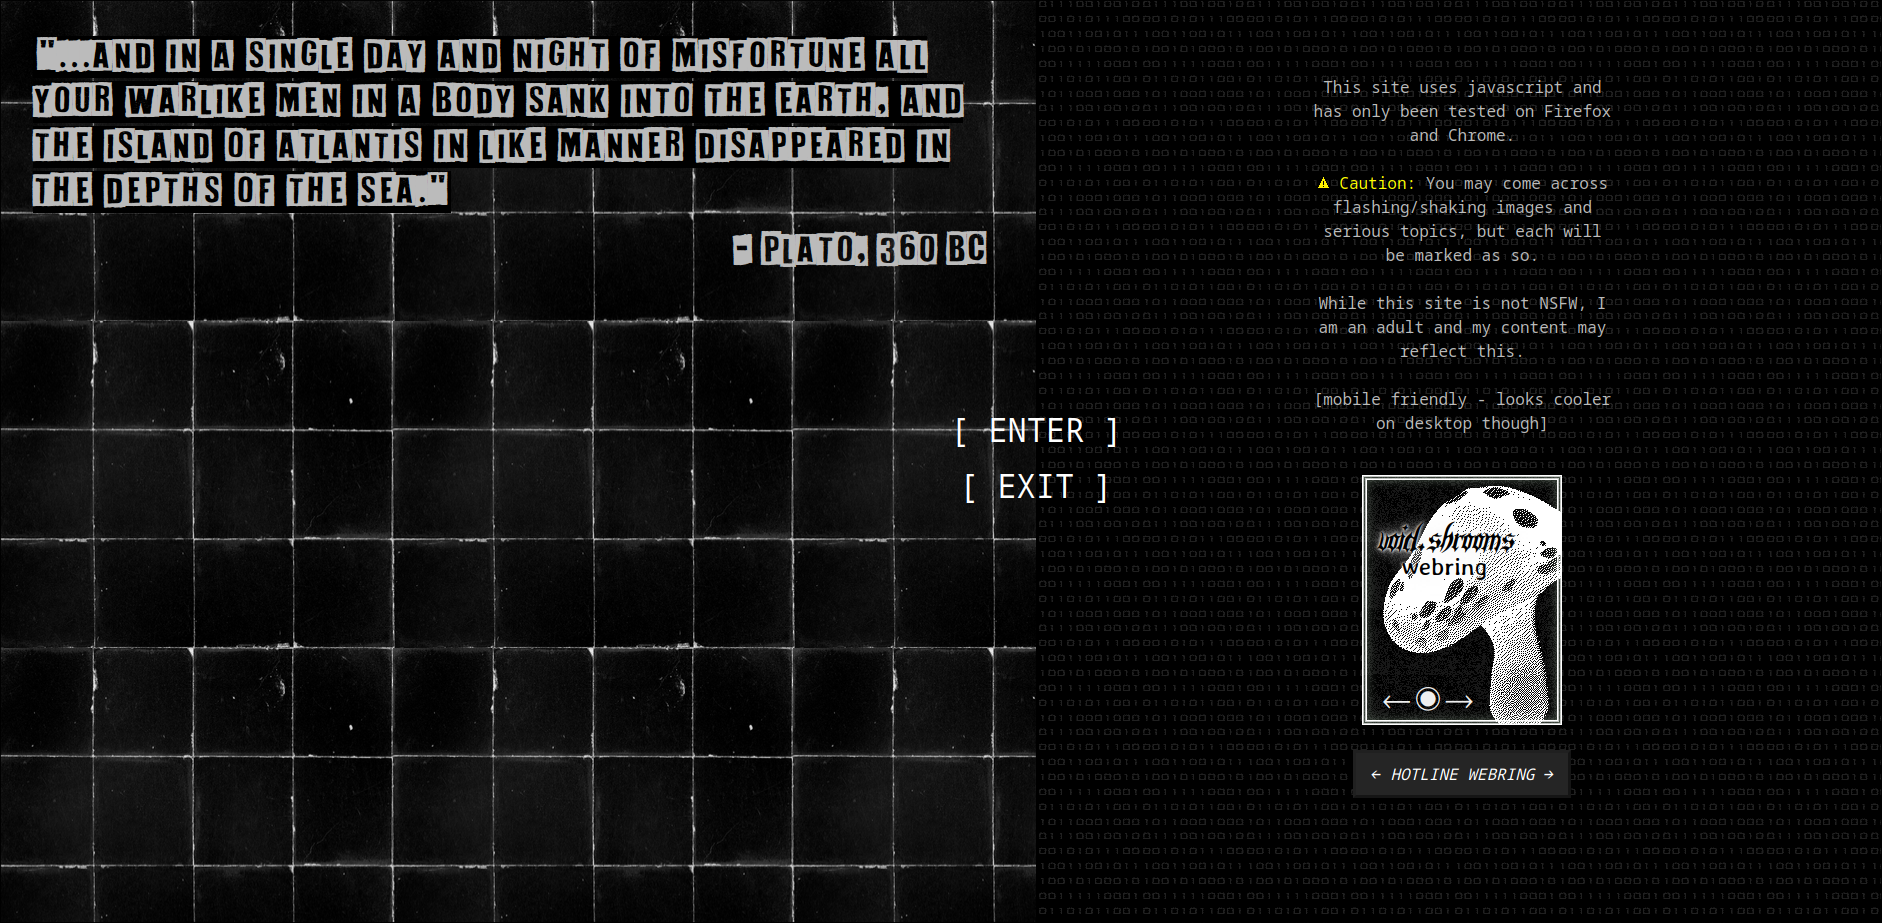
\includegraphics[scale=0.1]{website3.png}
    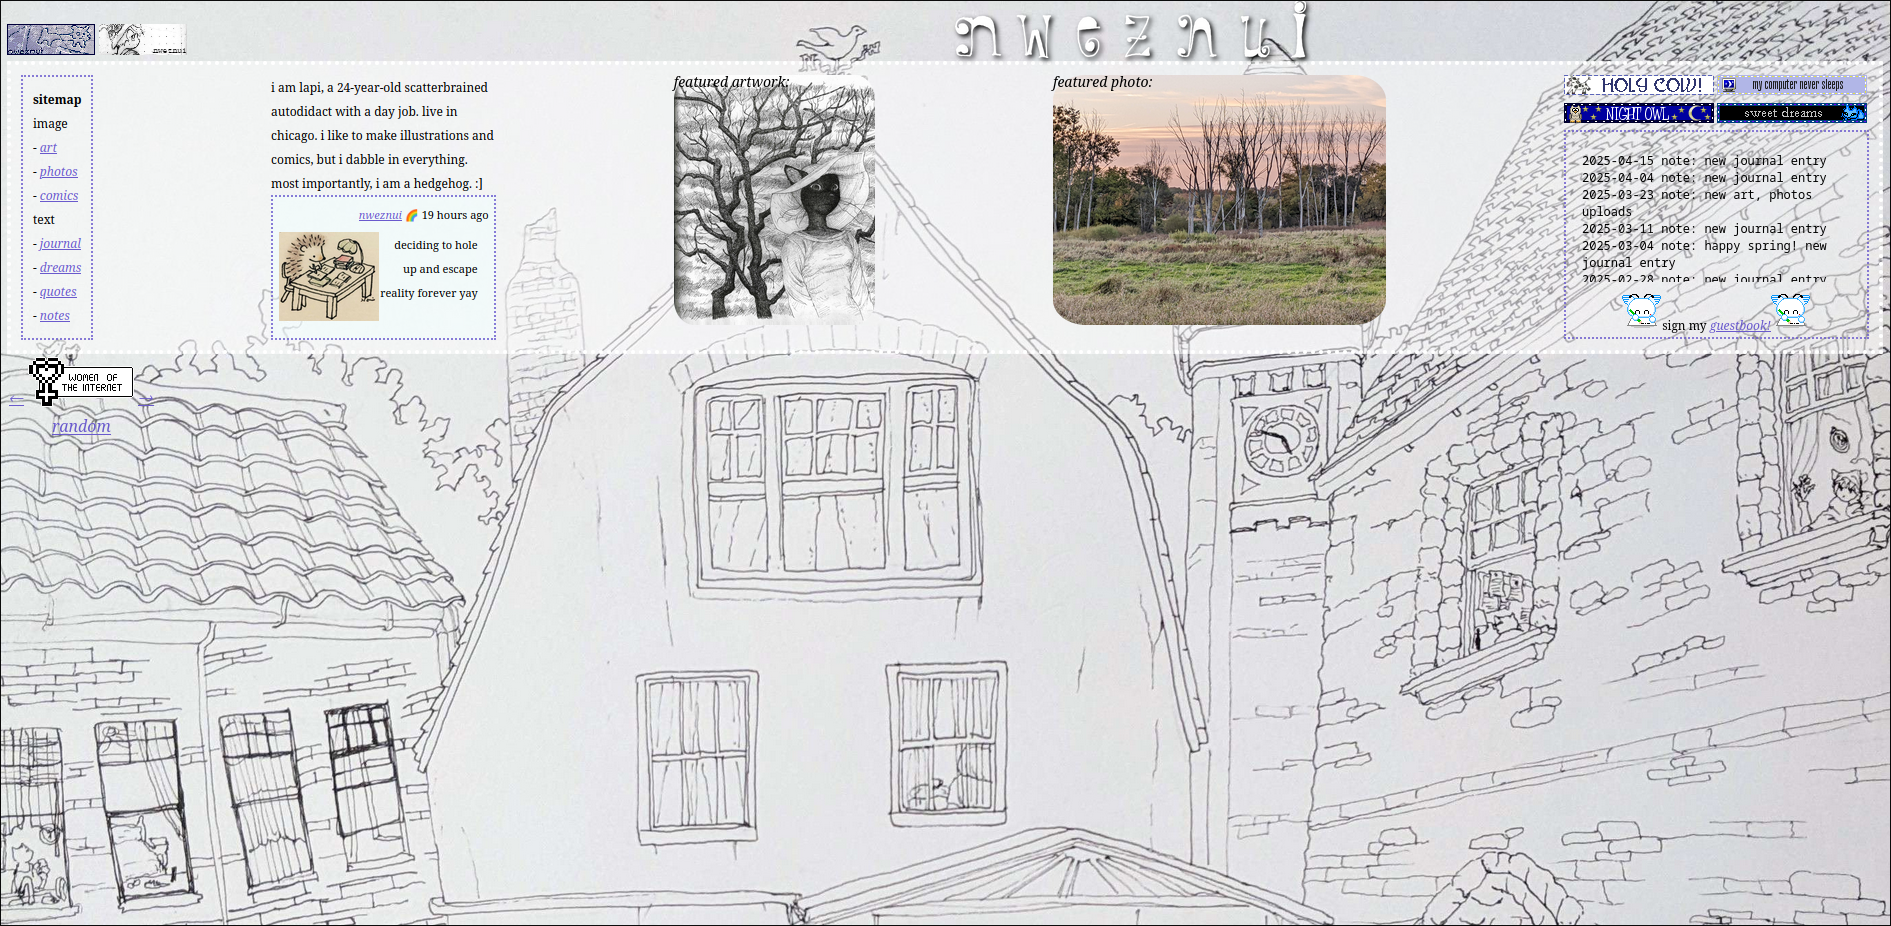
\includegraphics[scale=0.1]{website5.png}
  \end{center}
\end{frame}

\begin{frame}{Designing}
\centering
\begin{figure}[h!]
    \begin{subfigure}{0.4\textwidth}
      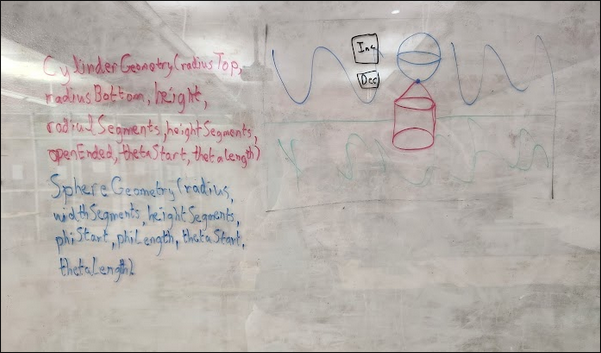
\includegraphics[width=1\textwidth]{whiteboard1.png}
      \caption*{My initial design for this balloon project}
    \end{subfigure}
    \begin{subfigure}{0.4\textwidth}
      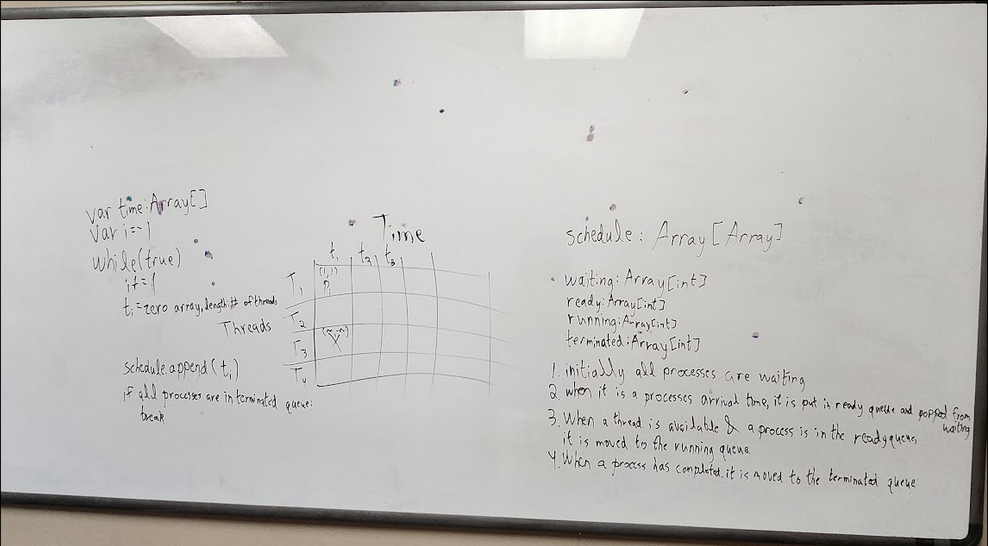
\includegraphics[width=1\textwidth]{whiteboard2.png}
      \caption*{My design for my CPU Scheduling algorithm}
    \end{subfigure}
\end{figure}
\end{frame}


\begin{frame}{HTML}
  HTML creates the objects on our website.
  \centering
  \begin{figure}
    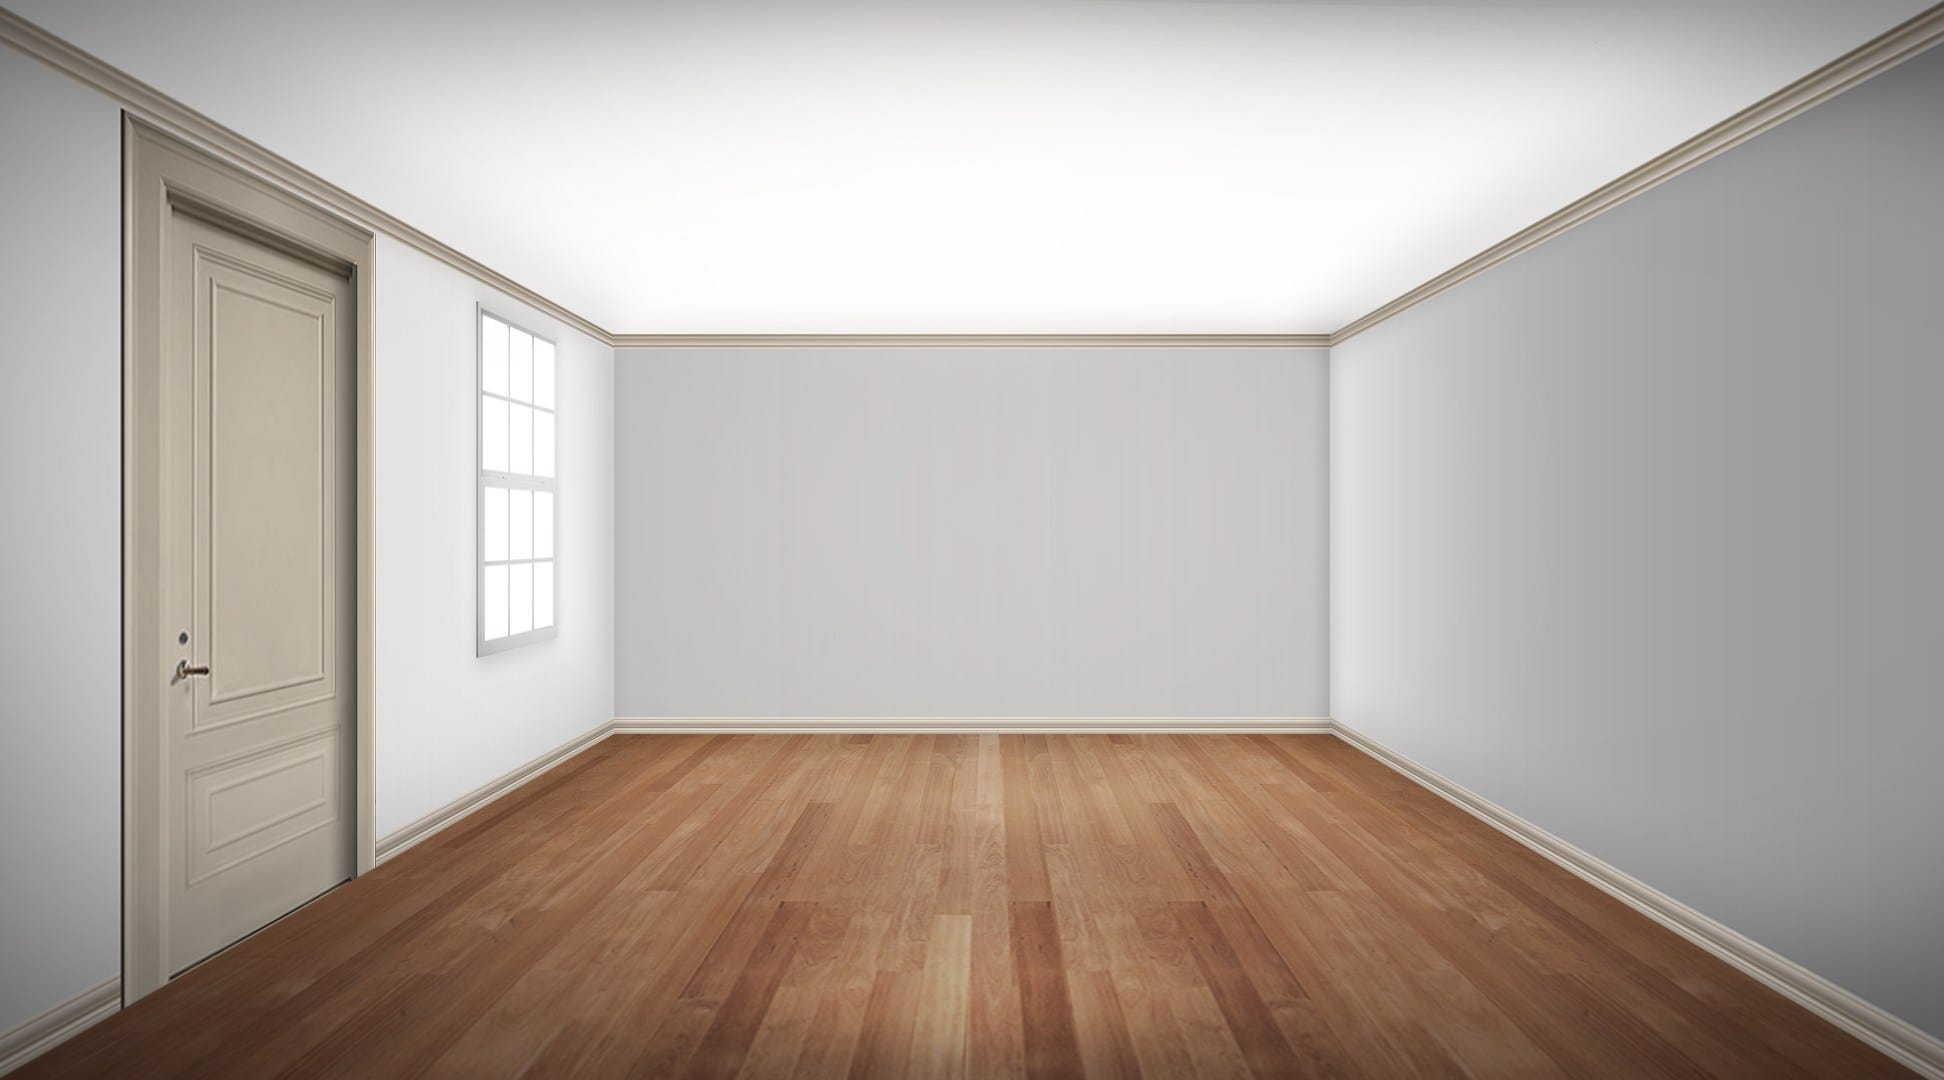
\includegraphics[scale=0.12]{emptyHouse.jpg}
    \caption*{\small You can think of it as an empty house, a place with structure but no decoration.}
  \end{figure}
\end{frame}

\begin{frame}{CSS}
  CSS customizes our objects from HTML.
  \centering
  \begin{figure}
    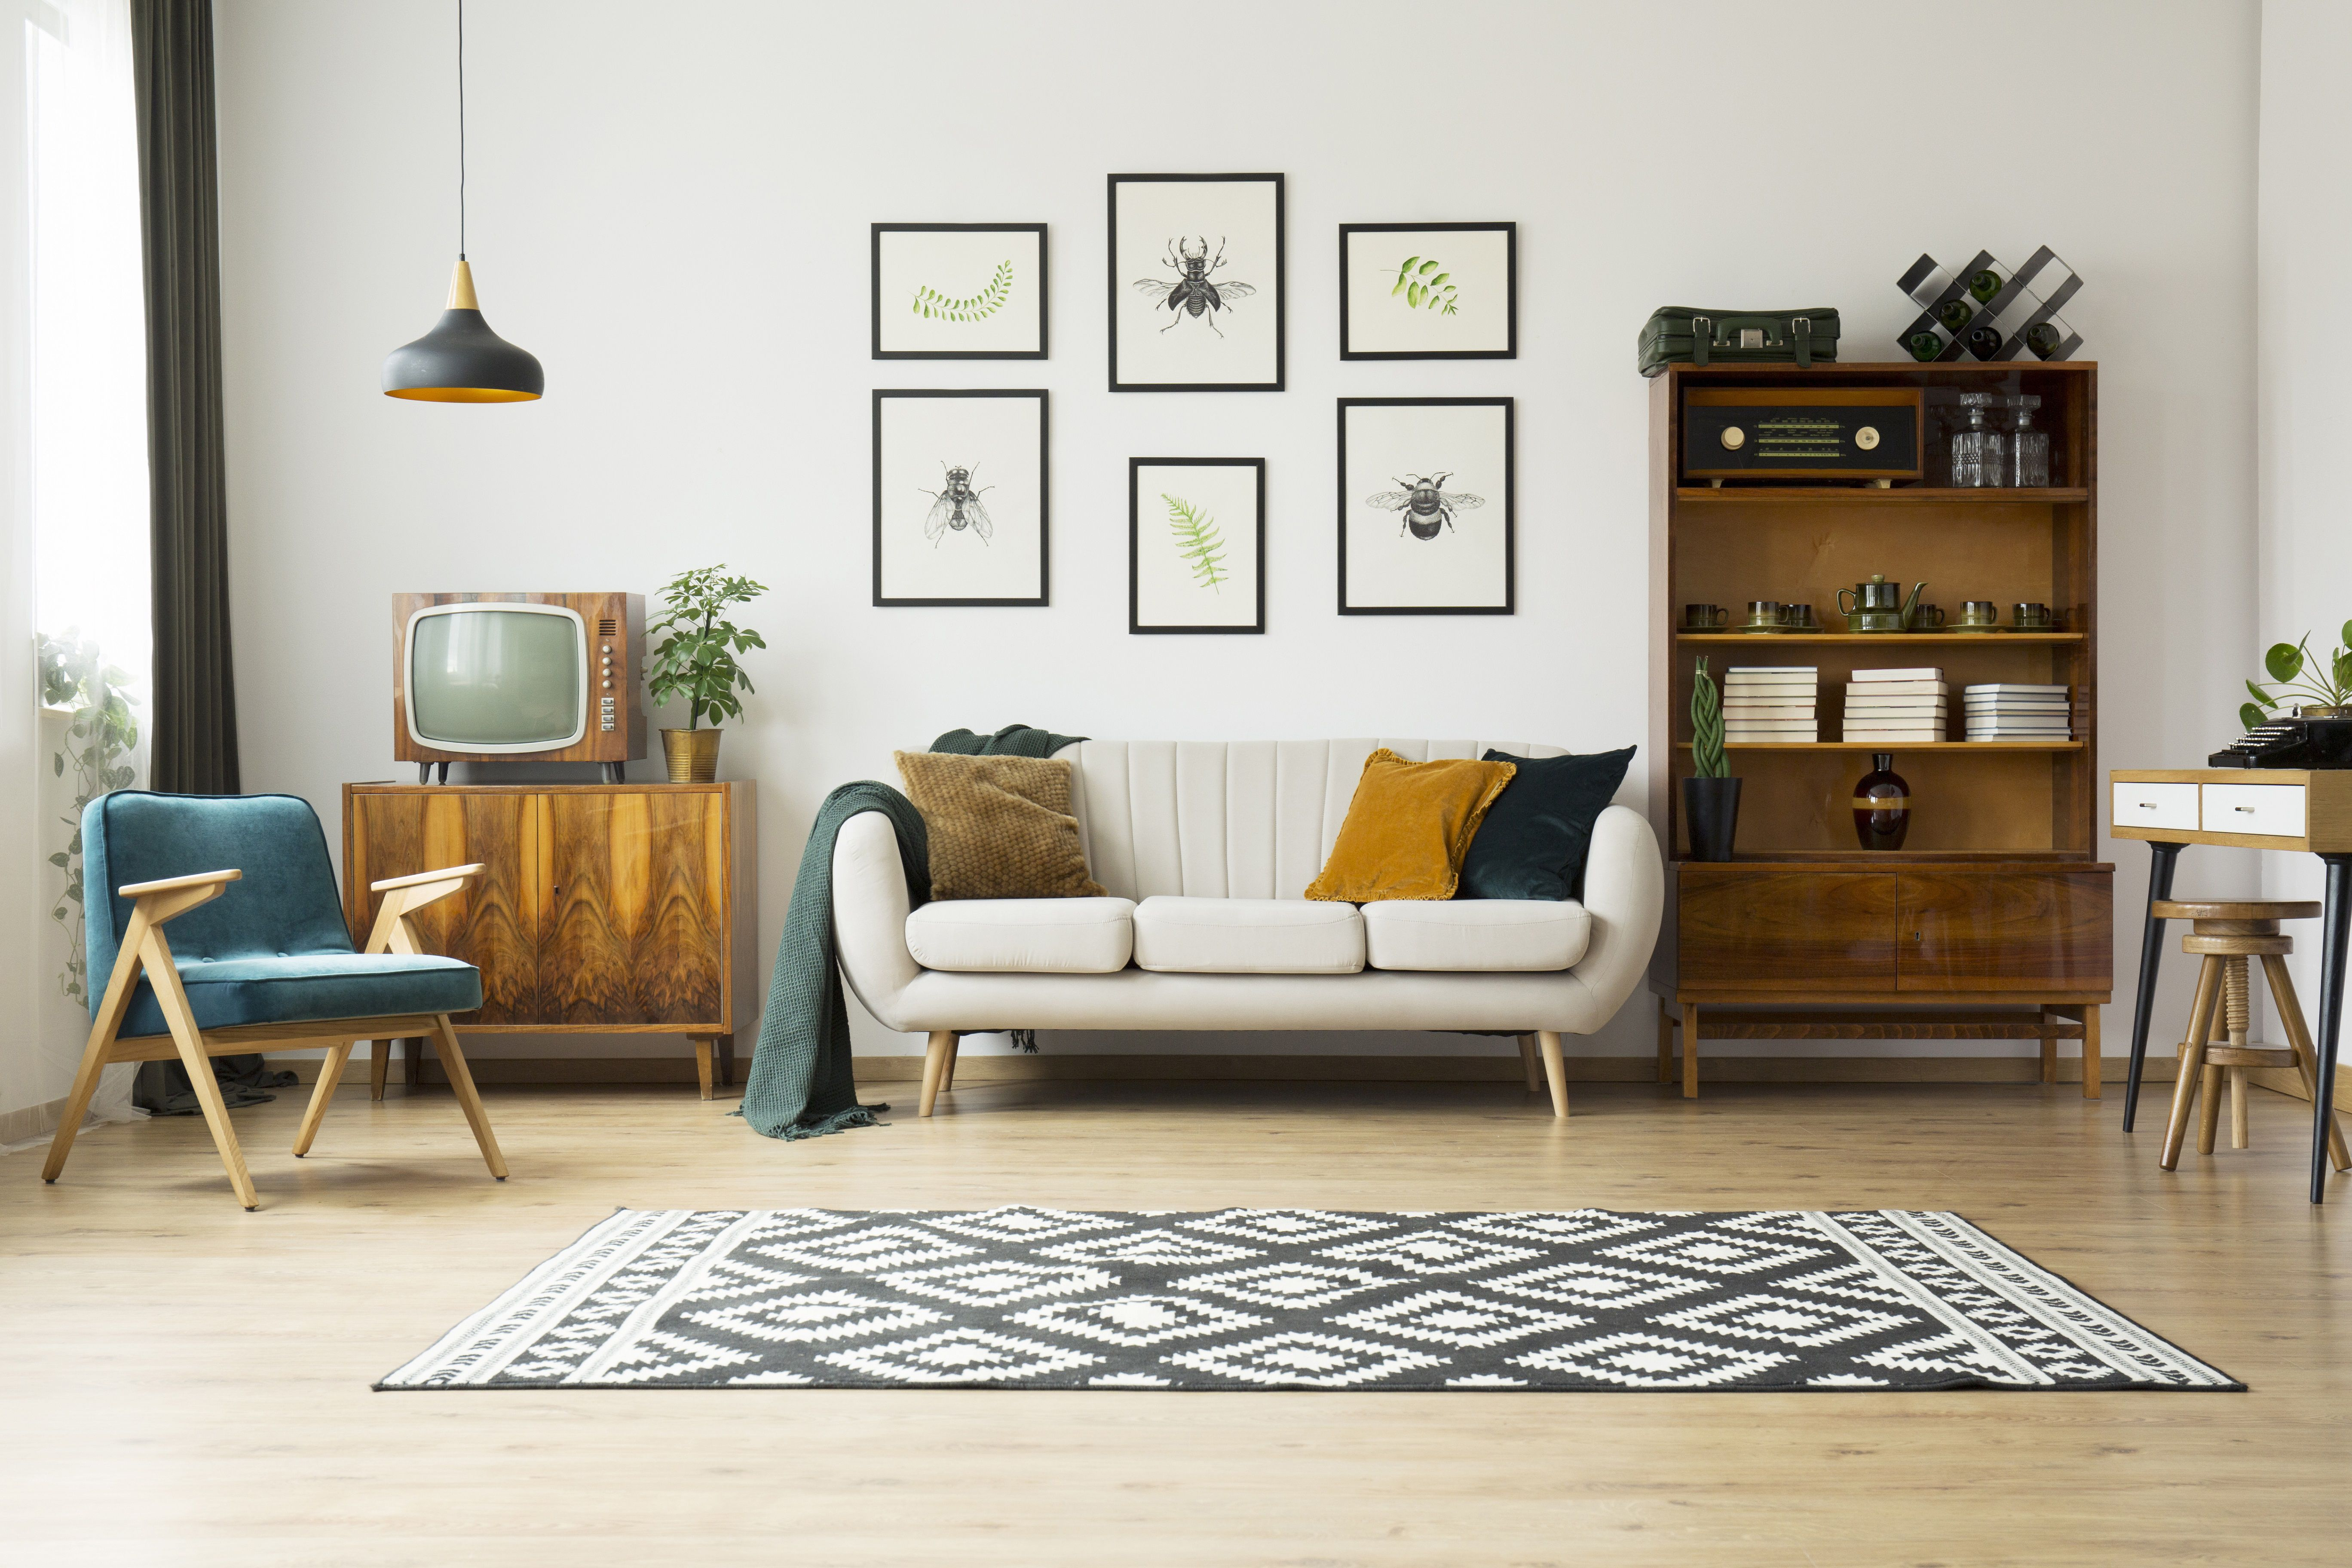
\includegraphics[scale=0.04]{decoratedHouse.jpg}
    \caption*{This decorates our house with color, animations, etc.}
  \end{figure}
\end{frame}

\begin{frame}{Hosting}
\centering
\begin{figure}[h!]
    \begin{subfigure}{0.4\textwidth}
      
\includegraphics[width=1\textwidth]{neocities.png}
      \caption*{\large Neocities}
    \end{subfigure}
    \begin{subfigure}{0.4\textwidth}
      
\includegraphics[width=1\textwidth]{Github.jpg}
      \caption*{\large Github Pages}
    \end{subfigure}
\end{figure}

\end{frame}

\begin{frame}
  \center
  \Huge
  Questions?
\end{frame}

\begin{frame}
  \center
  \Huge
  Homework Questions
\end{frame}

\end{document}
